%!TEX program = lualatex
% LTeX: language=de-DE
\documentclass{beamer}
\usepackage[utf8]{luainputenc}
\usepackage{emoji}
\usepackage[
	typ=ohne,
	fach=Informatik,
	zitate=quotes,
	lerngruppe=6,
	lizenz=cc-by-sa-4,
	farbig,
	module={Symbole, Lizenzen, Papiertypen}
]{schule}
\usetheme{metropolis}

\usepackage{qrcode}

\usepackage{adjustbox}
% Fancy fit image command with optional caption
\makeatletter
\newcommand{\fitimage}[2][\@nil]{
  \begin{figure}
    \begin{adjustbox}{width=0.9\textwidth, totalheight=\textheight-2\baselineskip-2\baselineskip,keepaspectratio}
      \includegraphics{#2}
    \end{adjustbox}
    \def\tmp{#1}%
   \ifx\tmp\@nnil
      \else
      \caption{#1}
    \fi
  \end{figure}
}
\makeatother

\setbeamertemplate{frame footer}{v20223-12-17 \hfill \lizenzSymbol}


\title{B6-Code}
\subtitle{Codieren von Daten}
\date{}


\begin{document}
\frame{\titlepage}

\begin{frame}
	\begin{figure}
    \centering
    \fitimage{5515626016_1a37c22695_c.jpg}
    \small{QR code DICE von \href{https://flickr.com/photos/marketrumba/}{Dianna Helm} unter der Lizenz \href{https://creativecommons.org/licenses/by/2.0/}{CC-BY 2.0} via \href{https://flickr.com/photos/marketrumba/5515626016/in/photolist-9pp2sh-bcdB5a-9uBSzB-9ns3Qb-5UEYNb-rLo6vW-efsAmU-2kKiRUZ-bhzmXe-2ozHt2Q-2ozGbeW-8NkYm7-2oARGMA-2ozJWRp-dZMsHs-2ozJx9b-7B2LMV-7PTnYd-acpiyT-a9Wk32-9m9eds-5tpEfb-2ozJZw4-dxyZQZ-9XJh81-9m9e7Y-2ozDf6R-65a4tp-5qsA45-9m9eau-adXWea-asmcJi-9fEV63-2mP9Fsr-8xAJxS-9TiyD3-7YYLbH-em3z1w-9q1yKt-dYnSL5-8crU4j-9fEUMG-81QJNR-ccQ6rL-oZ8zTh-2hSBXaf-2ozDf5i-2mQAthB-ajNoNY-AEx5nZ}{Flickr}}
	\end{figure}
  \tiny{Alternatives Bild: \url{https://www.adexchanger.com/wp-content/uploads/2020/12/comic_QR-codes_400.jpg}}
\end{frame}

\begin{frame}
  \centering
  \huge
  Wie funktionieren solche Codes?
  \\
  \vspace{0.5cm}
  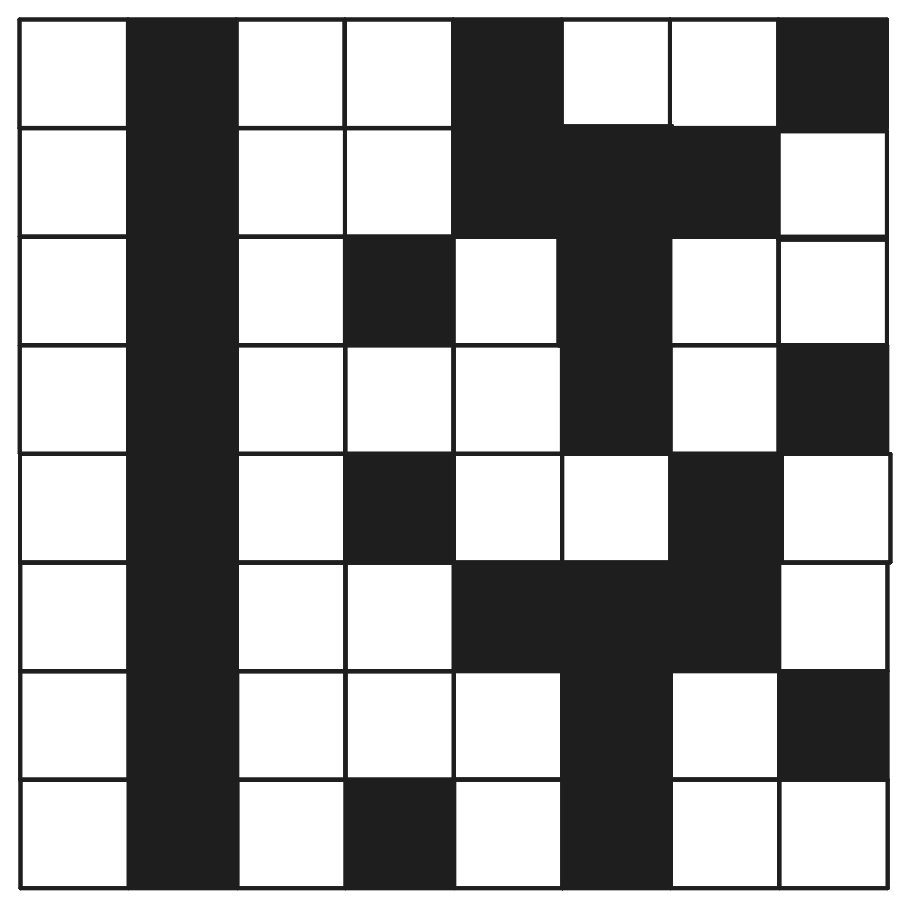
\includegraphics[width=0.3\textwidth]{./b6code-internet.excalidraw.png}
  \\
  \huge
  B6-Code
\end{frame}

\begin{frame}[t]
	\frametitle{Ablauf der Stunde}

	\begin{columns}[t]
		\begin{column}{0.3\textwidth}
			\centering
			\textbf{Phase: Weiß \emoji{white-circle}}
			Wie kann mit dem B6-Code ein Wort codiert und decodiert werden?
		\end{column}
		\begin{column}{0.3\textwidth}
			\centering
			\textbf{Phase: Blau \emoji{blue-circle}}
			Wie kann beim Dekodieren der Anfang des B6-Codes erkannt werden?
		\end{column}
		\begin{column}{0.3\textwidth}
			\centering
			\textbf{Phase: Grün \emoji{green-circle}}
			Wie kann der B6-Code robuster gemacht werden?
		\end{column}
	\end{columns}

	\begin{columns}
		\begin{column}{0.3\textwidth}
			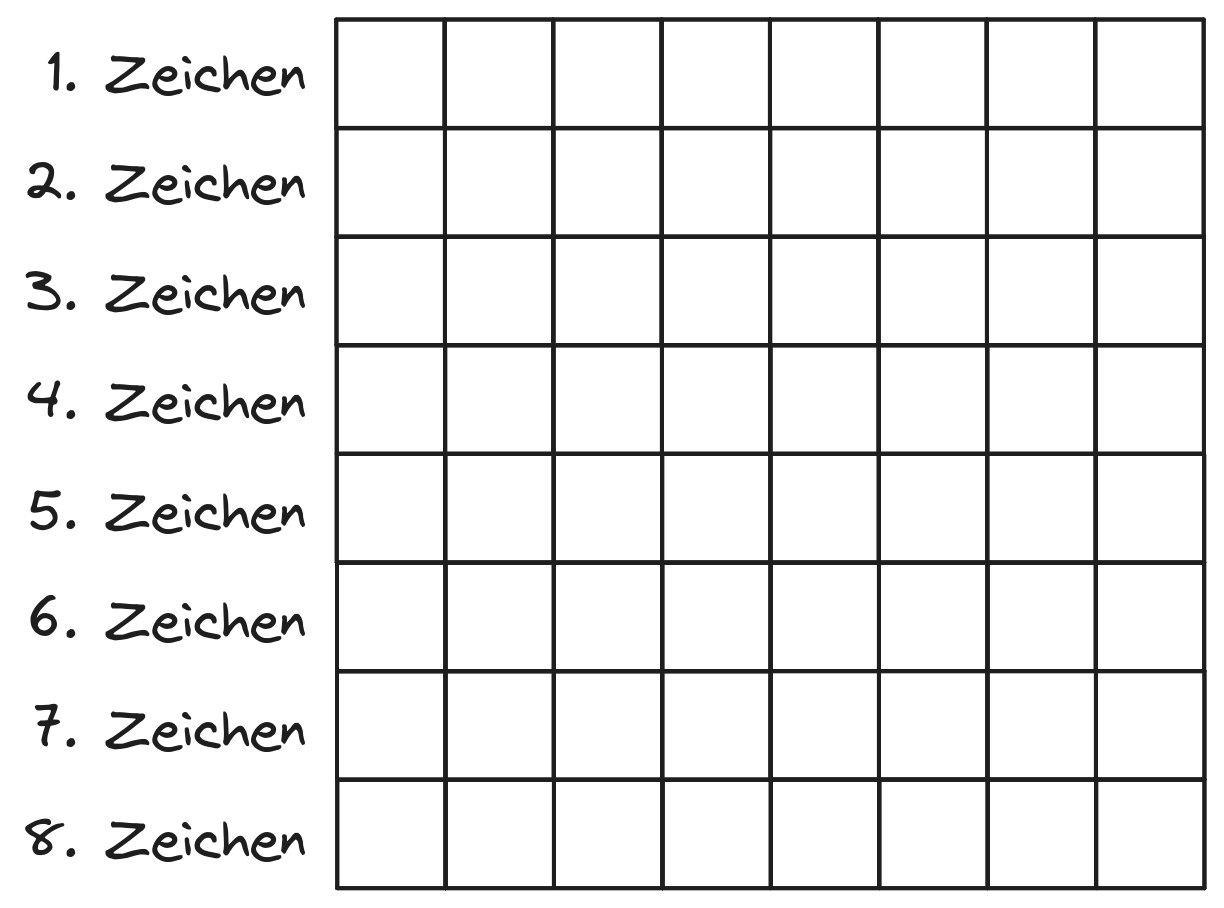
\includegraphics[width=\textwidth]{./b6code-struktur.excalidraw.png}
		\end{column}
		\begin{column}{0.3\textwidth}
			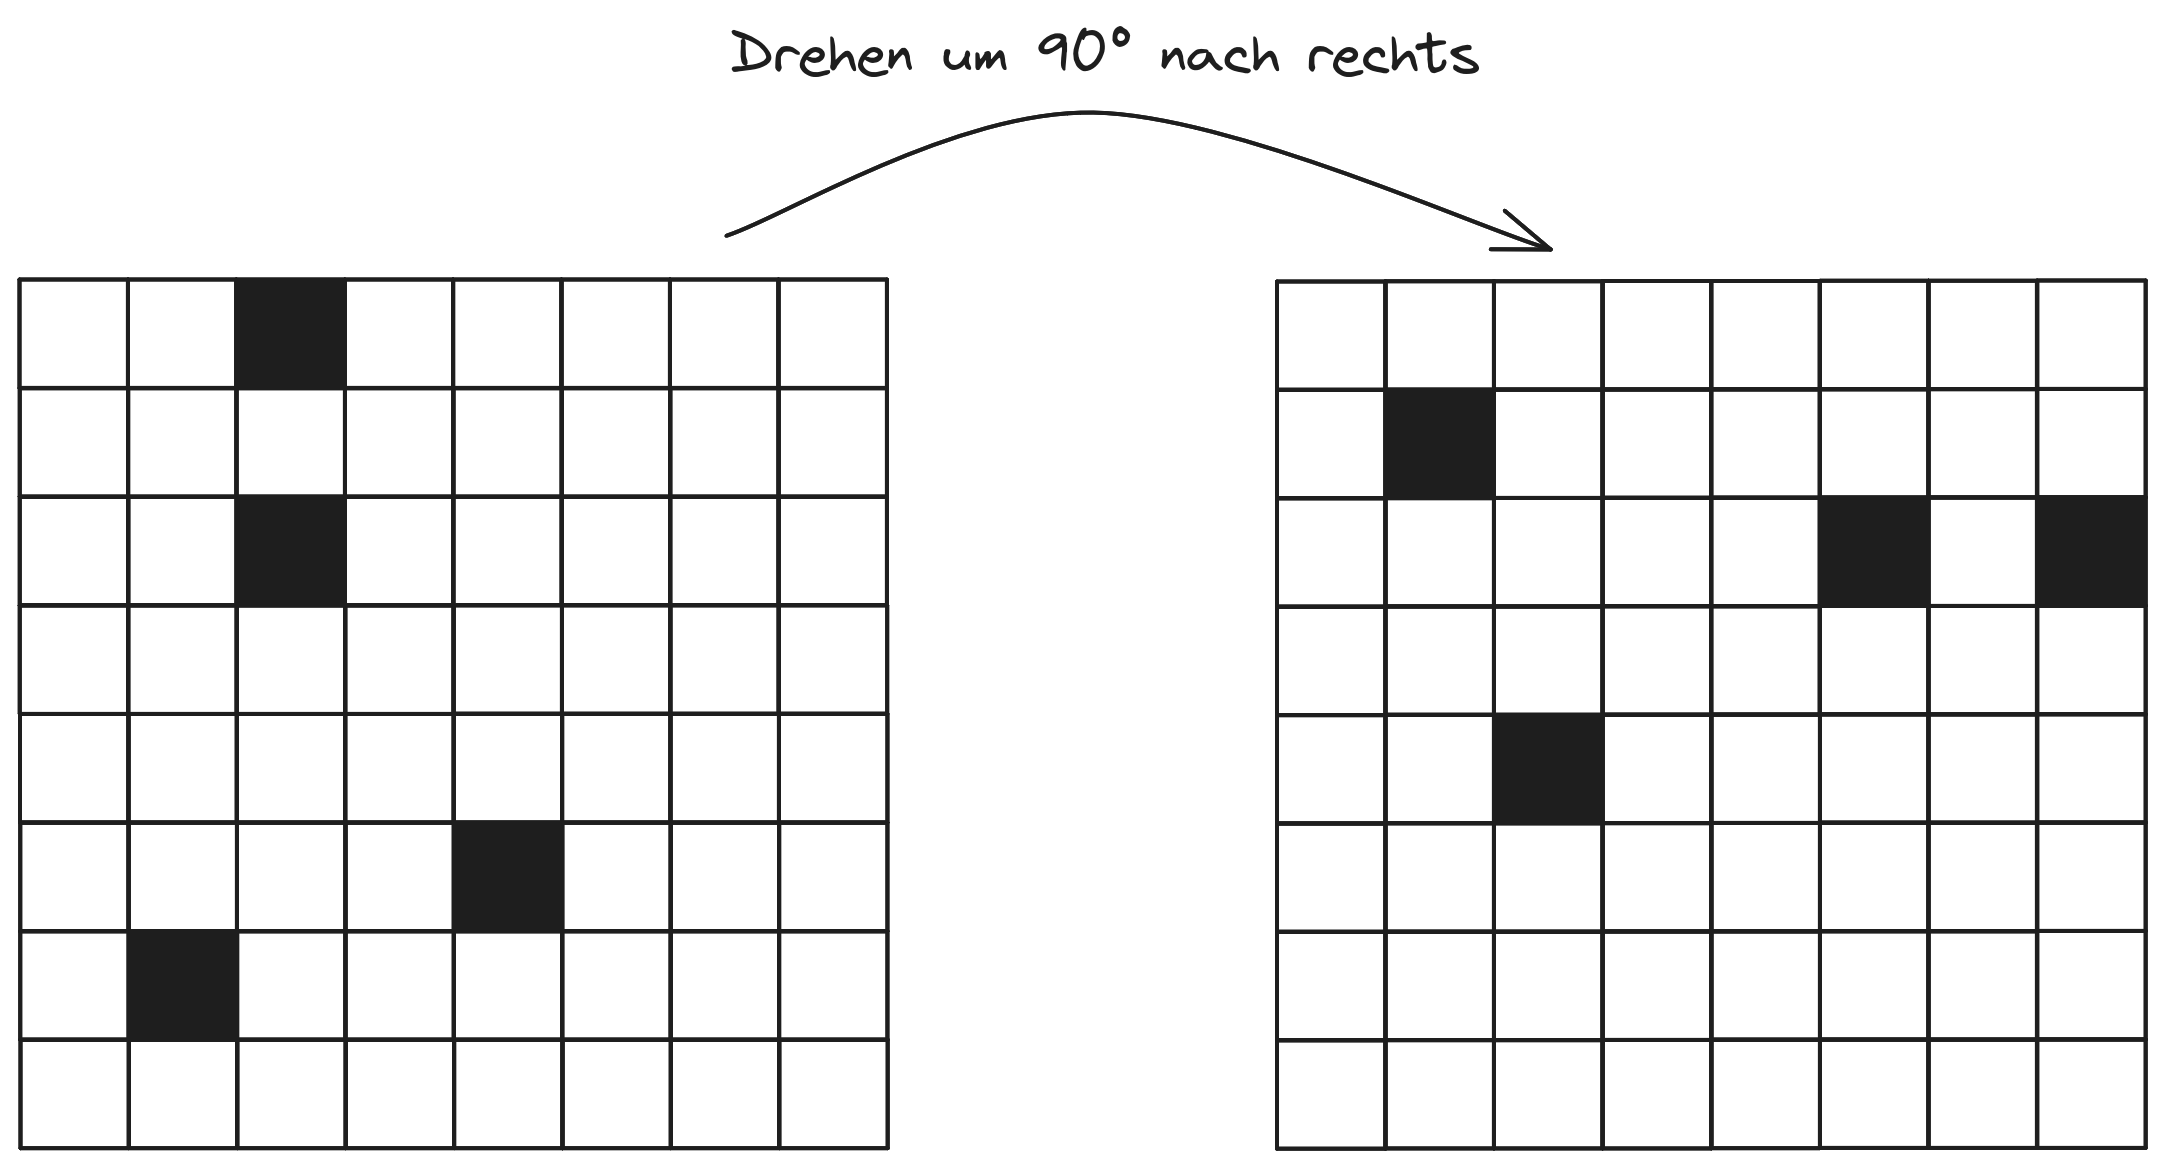
\includegraphics[width=\textwidth]{./b6code-drehen.excalidraw.png}
		\end{column}
		\begin{column}{0.3\textwidth}
			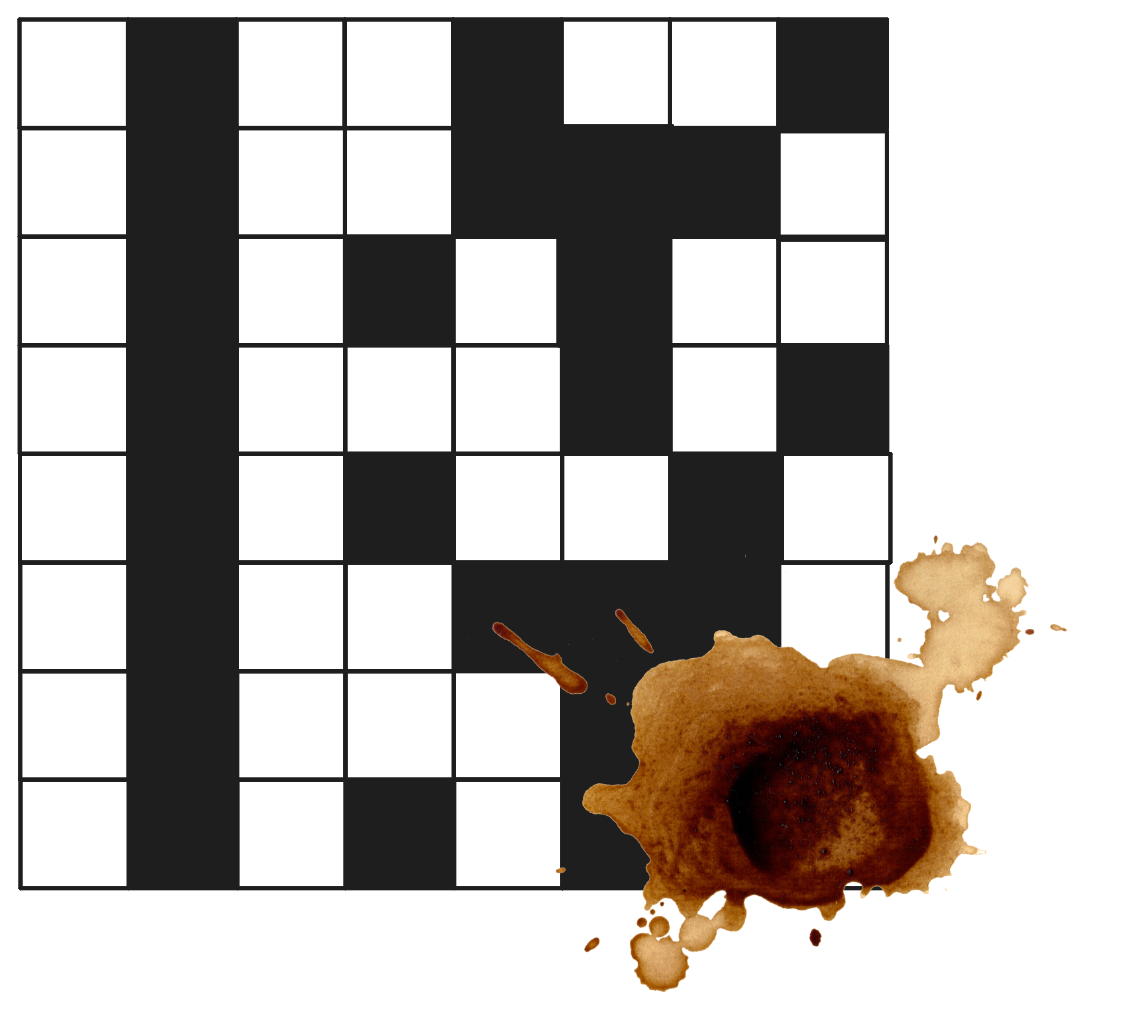
\includegraphics[width=\textwidth]{./b6code-fehler.excalidraw.png}
		\end{column}

	\end{columns}
\end{frame}

\begin{frame}
	\frametitle{\emoji{white-circle} Wie kann mit dem B6-Code ein Wort codiert und decodiert werden?}
\end{frame}

\begin{frame}
	\frametitle{\emoji{blue-circle} Wie kann beim Dekodieren der Anfang des B6-Codes erkannt werden?}
\end{frame}

\begin{frame}
	\frametitle{\emoji{green-circle} Wie kann der B6-Code robuster gemacht werden?}
\end{frame}

\begin{frame}
	\frametitle{Der QR-Code}
	\begin{center}
		\qrcode{https://duckduckgo.de}
	\end{center}
\end{frame}

\end{document}
